\section{Анализ структуры данных видеоконвейера}

Для построения эффективной модели прогнозирования необходимо провести анализ структуры и характеристик доступных данных. Исходный набор данных представляет собой многомерный временной ряд, собираемый системой мониторинга Prometheus [2] с различных компонентов видеоконвейера с периодичностью 15 секунд.

\subsection{Описание набора метрик}

Система мониторинга Prometheus [2] собирает широкий спектр метрик, характеризующих работу различных подсистем видеоконвейера, включая метрики ML-конвейера ($vidcap\_delay$, $vidcap\_fps$), бэкенда \\
($ml\_to\_backend\_kafka\_delay$, $db\_insert\_delay$), и WebSocket-клиентов \\
($heartbeat\_*$, $event\_counter$, $seq\_events\_health$).

Для построения модели прогнозирования отобраны следующие ключевые метрики, наиболее релевантные для задачи предсказания end-to-end-задержки:

\begin{itemize}
	\item $common\_cad$ --- целевая метрика end-to-end-задержки, усредненная за 1 час (мс);
	\item $db\_insert\_cad$ --- задержка записи в базу данных, усредненная за 1 час (мс);
	\item $kafka\_network\_cad$ --- сетевая задержка Kafka [4], усредненная за 1 час (мс);
	\item $counter\_events\_total$ --- общий счетчик обработанных событий в системе.
\end{itemize}

\subsection{Временные характеристики данных}

Исходный набор данных охватывает период с 25 ноября по 11 декабря 2024 года (16 дней непрерывной работы системы) и содержит 90543 временных точек. При интервале дискретизации 15 секунд это соответствует полному покрытию анализируемого периода без пропусков в данных.

\begin{figure}[H]
	\centering
	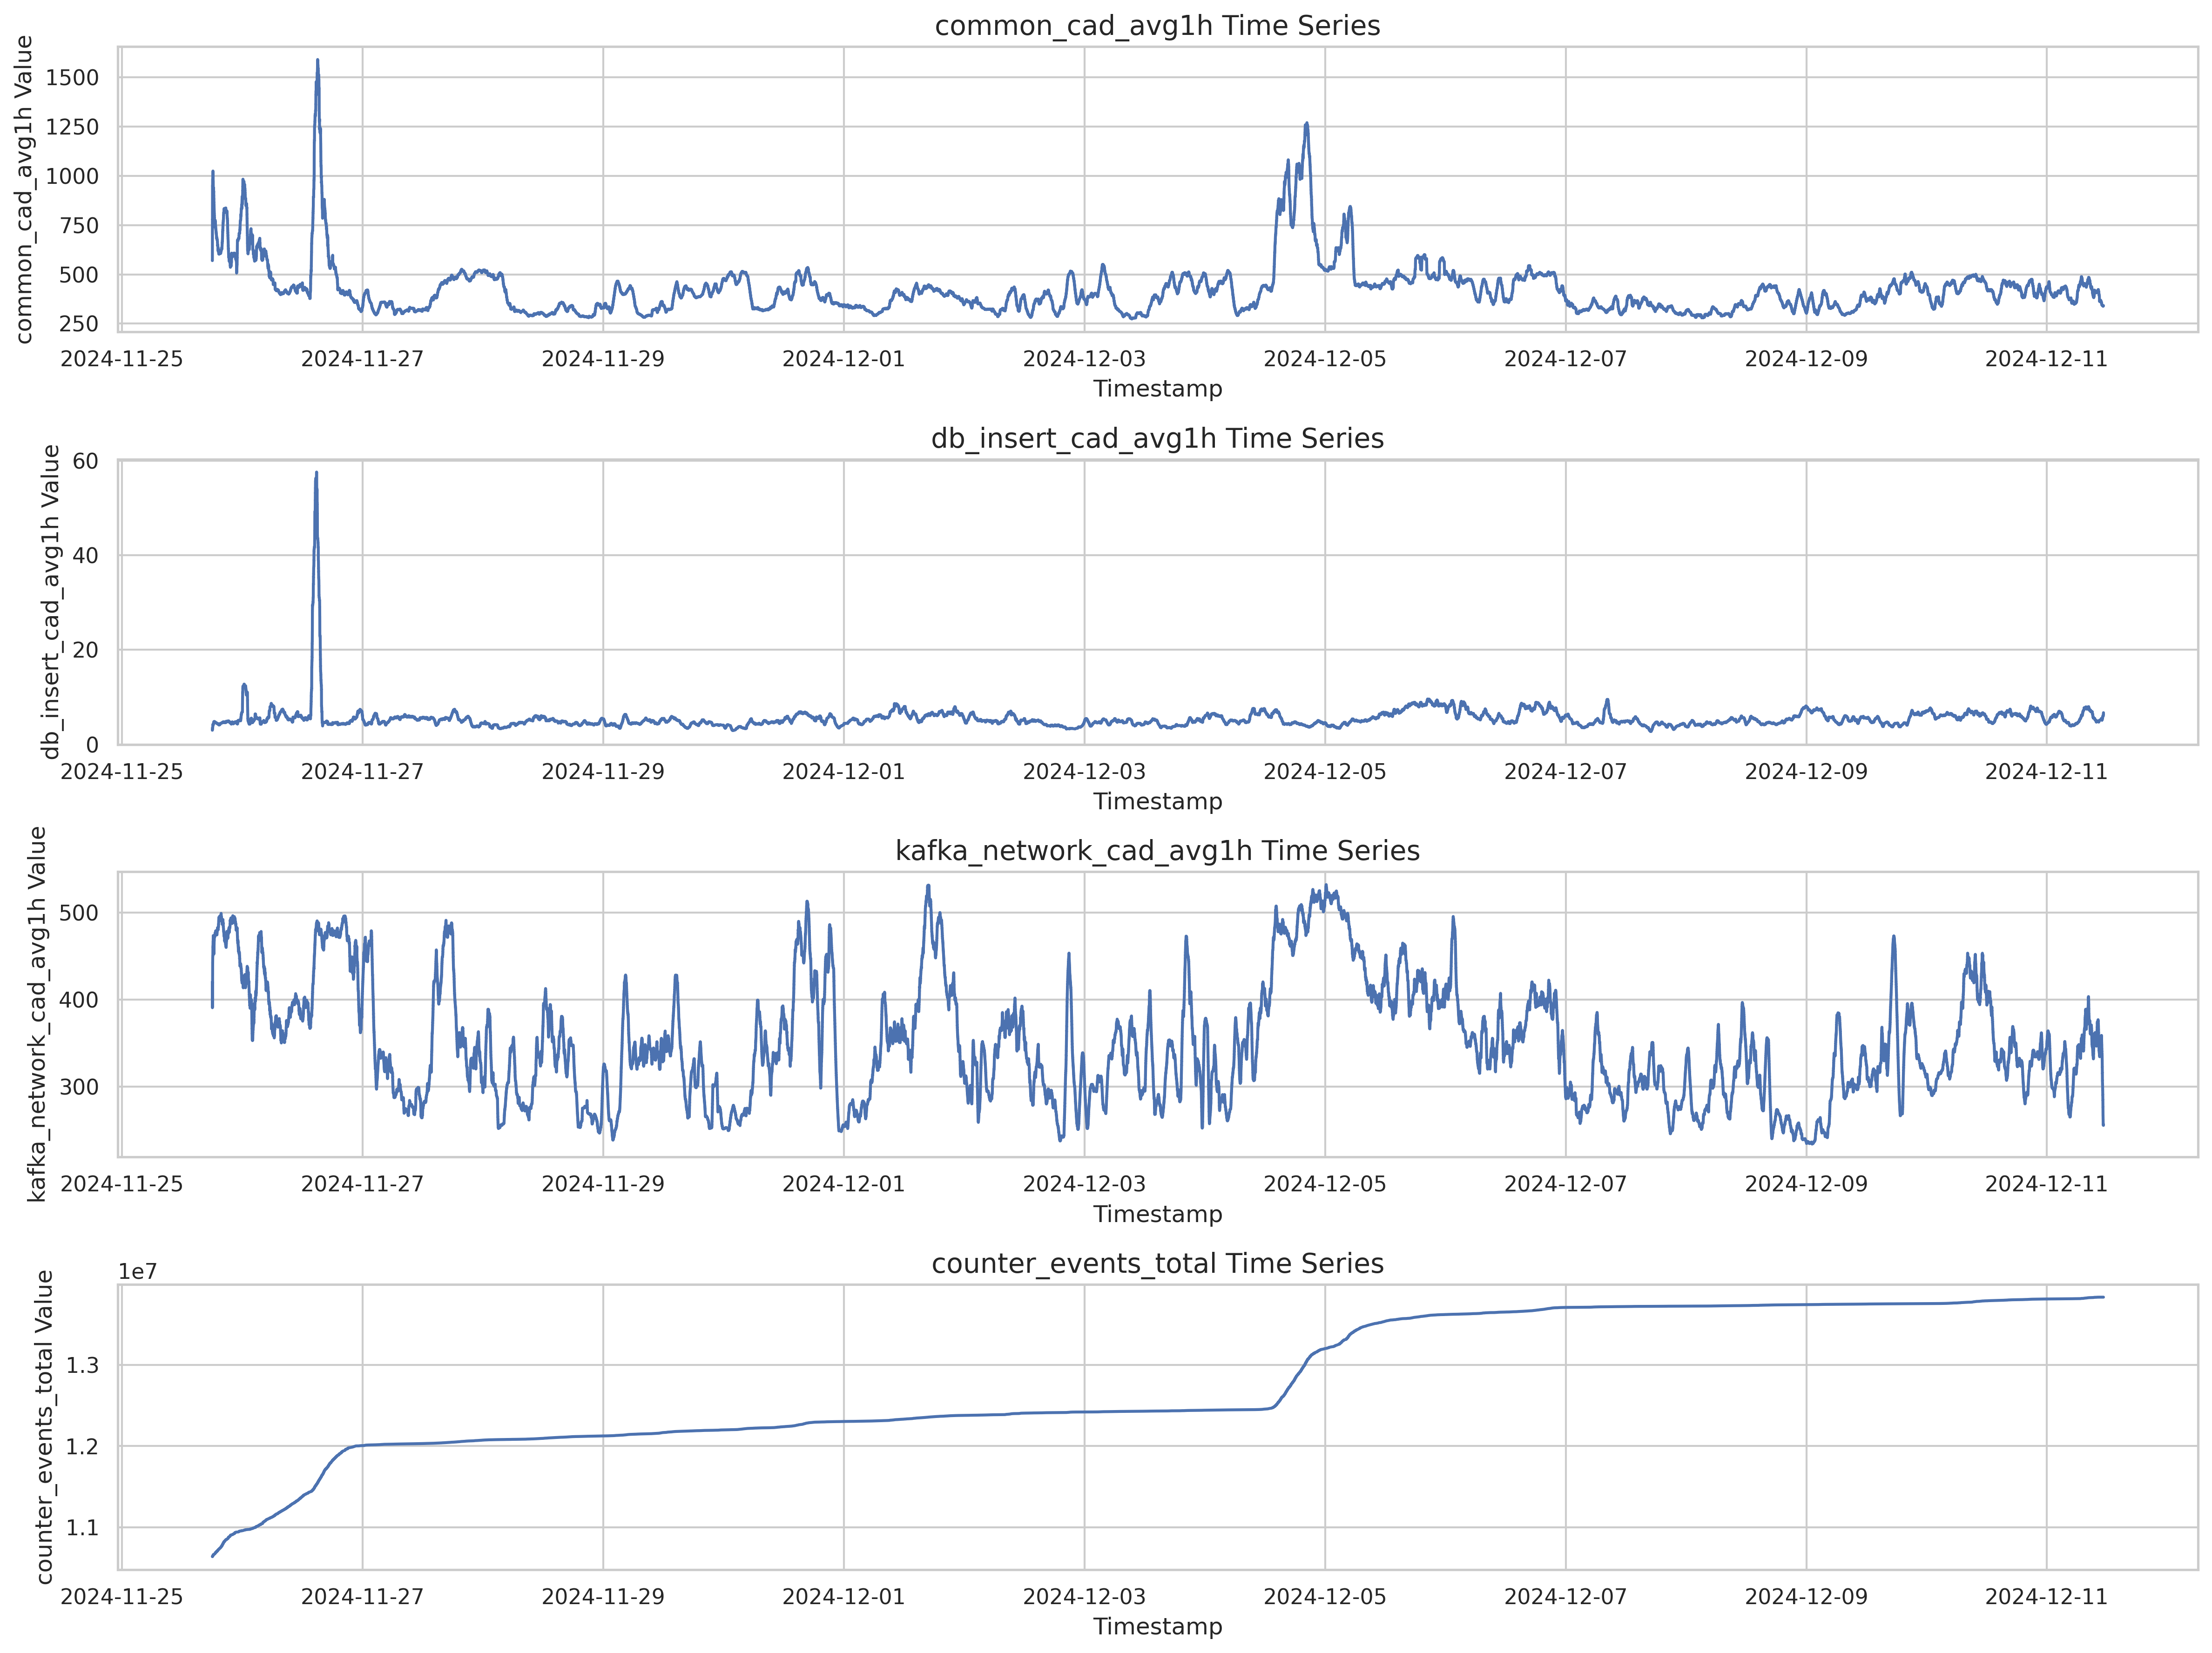
\includegraphics[width=0.9\textwidth]{figures/chapter2/time_series_overview.png}
	\caption*{Рисунок~2.1 --- Обзор временных рядов основных метрик видеоконвейера}
	\label{fig:time_series_overview}
\end{figure}

Анализ временных характеристик, представленных на \textit{рисунке 2.1}, показывает наличие различных паттернов в поведении метрик: циклические колебания, связанные с суточной активностью системы, периодические всплески нагрузки и редкие аномальные события, требующие особого внимания при построении модели.

\subsection{Статистический анализ метрик}

Для понимания распределения значений каждой метрики проведен описательный статистический анализ, результаты которого представлены в таблице 2.1.

\begin{table}[H]
	\centering
	\caption*{Таблица 2.1 --- Описательная статистика основных метрик}
	\begin{tabular}{|l|c|c|c|c|c|}
		\hline
		\textbf{Метрика} & \textbf{Среднее} & \textbf{Медиана} & \textbf{Мин.} & \textbf{Макс.} & \textbf{Std} \\
		\hline
		common\_cad & 423.72 & 400.63 & 273.66 & 1591.18 & 138.11 \\
		db\_insert\_cad & 5.51 & 5.07 & 2.74 & 57.56 & 2.73 \\
		kafka\_network\_cad & 351.51 & 339.84 & 234.22 & 532.15 & 68.76 \\
		counter\_events\_total & 1.28$\times$10$^{7}$ & 1.24$\times$10$^{7}$ & 1.06$\times$10$^{7}$ & 1.38$\times$10$^{7}$ & 8.21$\times$10$^{5}$ \\
		\hline
	\end{tabular}
	\label{tab:descriptive_stats}
\end{table}

\begin{figure}[H]
	\centering
	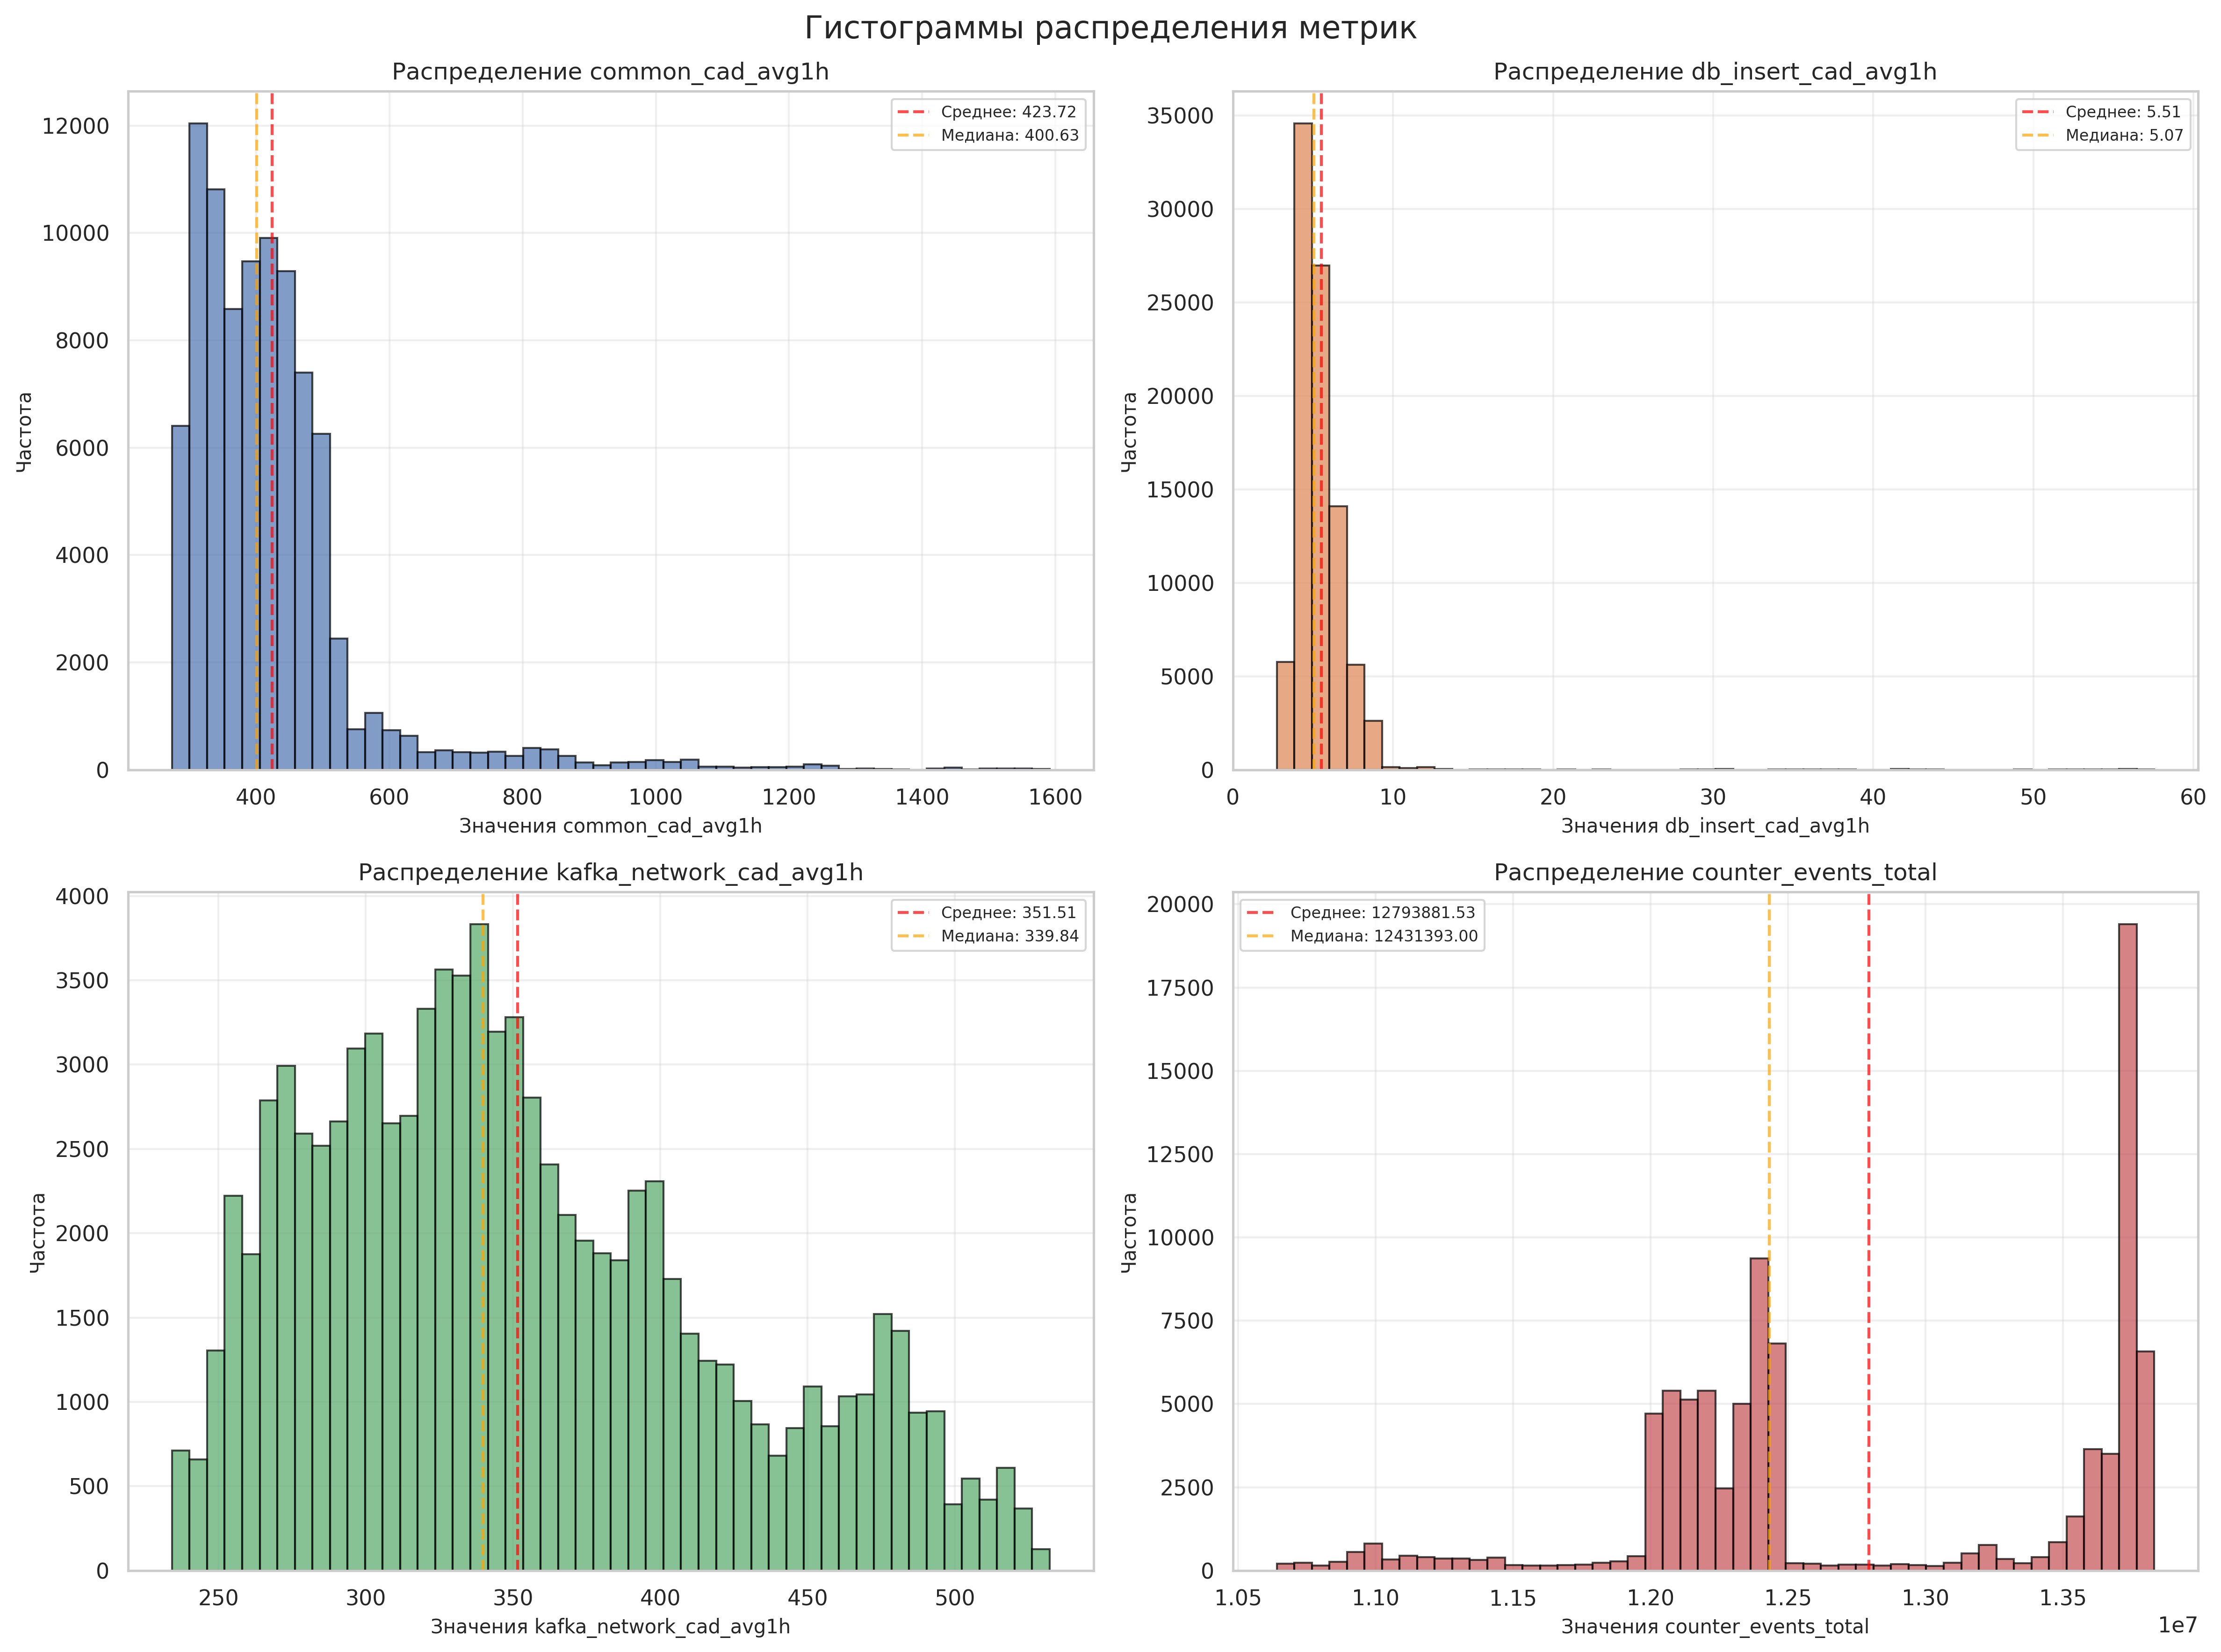
\includegraphics[width=0.9\textwidth]{figures/chapter2/metrics_distribution.png}
	\caption*{Рисунок~2.2 --- Гистограммы распределения ключевых метрик системы}
	\label{fig:metrics_distribution}
\end{figure}

На \textit{рисунке 2.2} представлены гистограммы распределения, которые показывают, что большинство метрик имеют распределение, близкое к нормальному, но со смещением и тяжелыми хвостами, что указывает на наличие выбросов.

\subsection{Анализ пропусков и качества данных}

Качество исходных данных является критическим фактором для построения надежной прогностической модели. Анализ показывает наличие пропусков данных только в начале и конце временных рядов, что связано с особенностями синхронизации сбора различных метрик. В середине периода наблюдения пропуски отсутствуют, что свидетельствует о стабильной работе системы мониторинга.

Для обеспечения единообразия временных рядов из каждой метрики было исключено следующее количество точек:

\begin{itemize}
	\item $common\_cad$ --- 2 точки;
	\item $db\_insert\_cad$ --- 188 точек;
	\item $kafka\_network\_cad$ --- 188 точек;
	\item $counter\_events\_total$ --- 216 точек.
\end{itemize}

Данная стратегия обработки пропусков путем обрезания краевых значений является предпочтительной по сравнению с интерполяцией, поскольку сохраняет естественную структуру временных зависимостей в данных и исключает внесение искусственных артефактов в модель.

\subsection{Выявление аномалий в данных}

Для обнаружения аномальных значений в данных применен метод межквартильного размаха (IQR). Точки, выходящие за границы $Q_1 - 1.5 \times IQR$ и $Q_3 + 1.5 \times IQR$, рассматриваются как потенциальные выбросы.

\begin{figure}[H]
	\centering
	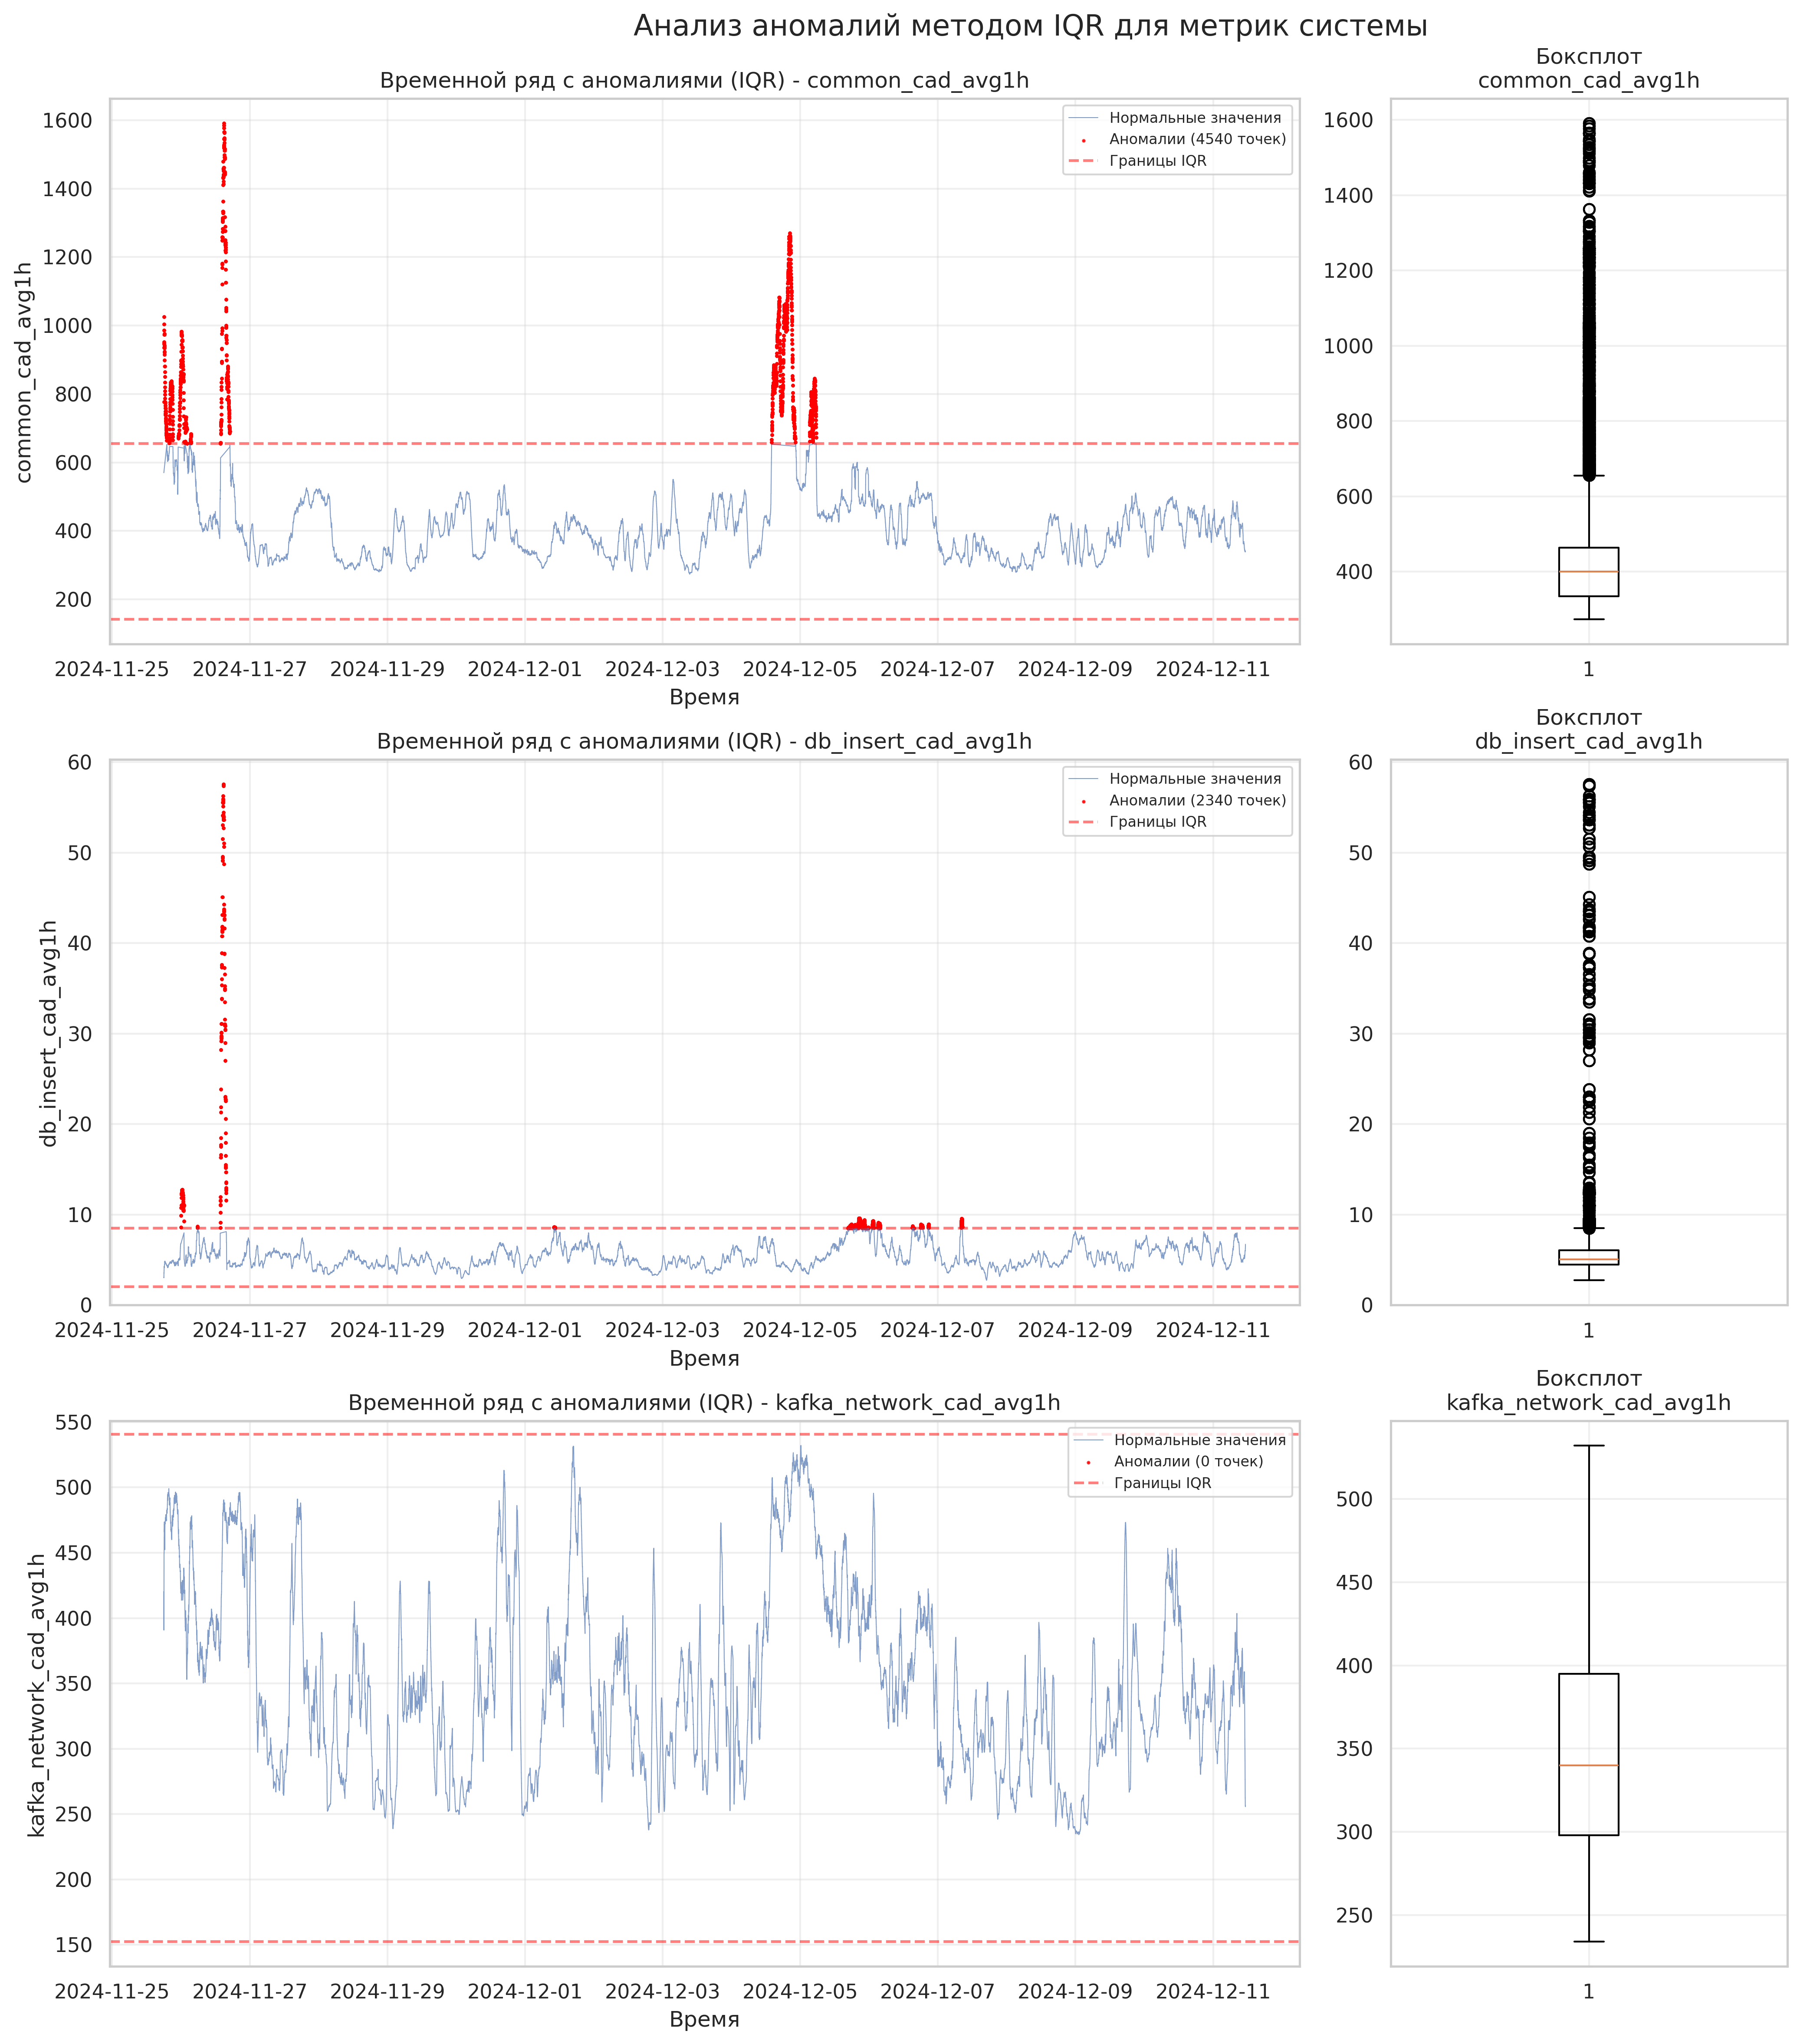
\includegraphics[width=0.9\textwidth]{figures/chapter2/outliers_boxplot.png}
	\caption*{Рисунок~2.3 --- IQR-диаграммы (диаграммы размаха) и boxplots для выявления выбросов в метриках}
	\label{fig:outliers_analysis}
\end{figure}

IQR-диаграммы на \textit{рисунке 2.3} наглядно демонстрируют квартили и выбросы для каждой метрики, позволяя оценить степень вариабельности данных и выявить аномальные периоды работы системы.

Обнаруженные аномалии требуют детального анализа для определения их природы: являются ли они результатом реальных событий в системе (пиковые нагрузки, сбои) или ошибками измерения. В зависимости от результатов анализа принимается решение о сохранении, корректировке или исключении аномальных точек из обучающей выборки. 